\section{Background and Motivation}\label{sec:motivation}

In this section, we first introduce how the language specification describes
JavaScript syntax and semantics of language features with simple examples.
%
Then, we explain how prior work~\cite{jest} synthesizes JavaScript conformance
tests using coverage-guided fuzzing~\cite{afl} with the control-flow graph (CFG)
in the language specification.
%
Finally, we explain why node/branch coverages cannot fully discriminate
different semantics in different language features or even in the same features.




\subsection{JavaScript Language Specification (ECMA-262)}

ECMA-262 is the official JavaScript language specification written in English
and maintained by the Ecma Technical Committee 39 (TC39).
%
Now, we explain how it describes JavaScript syntax and semantics of language
features with simple examples.




\subsubsection{Syntax}

\begin{figure}
  \centering
  \begin{subfigure}{\textwidth}
    \[
      \small
      \begin{array}{l}
        \esntp{AdditiveExpression}{Yield, Await} \est{:}\\

        \qquad \esntp{MultiplicativeExpression}{?Yield, ?Await}\\

        \qquad \esntp{AdditiveExpression}{?Yield, ?Await} \; \est{+} \;
        \esntp{MultiplicativeExpression}{?Yield, ?Await}\\

        \qquad \esntp{AdditiveExpression}{?Yield, ?Await} \; \est{-} \;
        \esntp{MultiplicativeExpression}{?Yield, ?Await}\\
      \end{array}
    \]
  \end{subfigure}
  \caption{
    The syntax of \esnt{AdditiveExpression} in ES13.
  }
  \label{fig:add-syntax}
\end{figure}

JavaScript syntax is defined with a variant of the extended Backus–Naur form
(EBNF).
%
It consists of syntactic productions defined with multiple alternatives, and
each alternative is a sequence of symbols.
%
Unlike the original EBNF, its nonterminals are parametric with boolean
arguments; $\esparam{?}$ denotes passing the argument as is, and $\esparam{+}$
and $\esparam{\(\sim\)}$ denote passing the \scode{true} and \scode{false},
respectively.
%
Beyond parametric nonterminals, it even provides context-sensitive symbols,
conditional alternatives, etc.
%
For example, consider the following simple additive expression:
%
\begin{equation}\label{equ:add}
  \jscode{1 + 2;}
\end{equation}
%
It tries to compute the addition of two Number values, \jscode{1} and
\jscode{2}.
%
Figure~\ref{fig:add-syntax} describes its syntax with the production of
\esnt{AdditiveExpression}.
%
It requires two boolean parameters, \esparam{Yield} and \esparam{Await}, and
consists of three alternatives.
%
The second (or third) one consists of three symbols, a nonterminal
\esnt{AdditiveExpression}, a terminal \est{+} (or \est{-}), and a nonterminal
\esnt{MultiplicativeExpression}.




\subsubsection{Semantics}

\begin{figure}
  \centering
  \begin{subfigure}{\textwidth}
    \small
    %----------------------------------------%
    $\fbox{\textsf{Syntax-directed operations (SDOs)}}$
    \vspace*{0.5em}\\
    %----------------------------------------%
    \textbf{Evaluation} of
    \esnt{AdditiveExpression} \est{:} \esnt{AdditiveExpression} \est{+}
    \esnt{MultiplicativeExpression}
    \\
    \null\quad 1. Return ?$\lab{2}$
    \esalg{EvaluateStringOrNumericBinaryExpression}$\lab{1}$(\esnt{AdditiveExpression},
    \escode{+}, \esnt{MultiplicativeExpression}).$\lab{3}$
    \vspace*{0.5em}\\
    %----------------------------------------%
    \textbf{Evaluation} of
    \esnt{AdditiveExpression} \est{:} \esnt{AdditiveExpression} \est{-}
    \esnt{MultiplicativeExpression}
    \\
    \null\quad 1. Return ?$\lab{5}$
    \esalg{EvaluateStringOrNumericBinaryExpression}$\lab{4}$(\esnt{AdditiveExpression},
    \escode{-}, \esnt{MultiplicativeExpression}).$\lab{6}$

  \end{subfigure}
  \caption{
    The semantics of \esnt{AdditiveExpression} defined with two syntax-directed
    operations (SDOs) in ES13.
  }
  \label{fig:add-sdo}
\end{figure}

The language specification describes semantics using abstract algorithms, and
there are three different kinds of abstract algorithms:
%
\begin{itemize}
  \item Syntax-directed operations (SDOs) (e.g., \textbf{Evaluation} of
    \esnt{AdditiveExpression} \est{:} $\cdots$ in Figure~\ref{fig:add-sdo})

  \item Normal algorithms (e.g., \textbf{ToNumeric} in
    Figure~\ref{fig:normal-algos})

  \item Built-in methods (e.g., \textbf{Number} in
    Figure~\ref{fig:builtin-number})
\end{itemize}

%----------------------------------------%

A \textit{syntax-directed operation (SDO)} defines the semantics of each
alternative in syntactic productions.
%
It consists of 1) target alternative, 2) name, 3) optional parameters, and 4)
body.
%
Each algorithm body is a pseudo-code consisting of well-organized steps written
in a natural language, English.
%
For example, two abstract algorithms in Figure~\ref{fig:add-sdo} are SDOs whose
target alternatives are the second and third ones of the
\esnt{AdditiveExpression} production for addition (\scode{+}) and subtraction
(\scode{-}) operators.
%
Their names are \textbf{Evaluation} with no optional parameters, and
bodies consist of a single step that invokes another normal algorithm
\textbf{EvaluateStringOrNumericBinaryExpression}.
%
Note that the variables \esnt{AdditiveExpression} and
\esnt{MultiplicativeExpression} in these SDOs store \textit{abstract syntax
trees (ASTs)} of the left- and right-hand side of given additive expressions.
%
For instance, if the first SDO in Figure~\ref{fig:add-sdo} takes the additive
expressions in~(\ref{equ:add}), two metavariables store ASTs of two Number
literals, \jscode{1} and \jscode{2}, respectively.
%
It means that abstract algorithms in ECMA-262 treat ASTs as values, and could
store them in variables or pass them as arguments of other algorithms.
%
The ``?'' operator is a shorthand for the following sequence of steps to handle
control flows:
\vspace*{.5em}\\
{
  \noindent
  \null\qquad 1. If \esvar{argument} is an abrupt completion, return
  \esalg{Completion}(\esvar{argument}).
  \\
  \null\qquad 2. Else if \esvar{argument} is a Completion Record, set
  \esvar{argument} to \esvar{argument}.[[Value]].
}
\vspace*{.5em}\\
where a completion record is \textit{abrupt} when it represents exceptional
control flows, such as \jscode{throw}, \jscode{return}, \jscode{break}, and
\jscode{continue}.
%
In other words, the ``?'' operator is a branch that checks whether given
values are abrupt completions and directly returns them if so.

%----------------------------------------%

\begin{figure}
  \centering
  \begin{subfigure}{\textwidth}
    \small
    %----------------------------------------%
    $\fbox{\textsf{Normal algorithms}}$
    \vspace*{0.5em}\\
    %----------------------------------------%
    \textbf{EvaluateStringOrNumericBinaryExpression} (
      \esvar{leftOperand},
      \esvar{opText},
      \esvar{rightOperand}
    )
    \\
    \null\quad $\lab{7}$...
    \\
    \null\quad 5. Return ?$\lab{9}$
    \esalg{ApplyStringOrNumericBinaryOperator}$\lab{8}$(\esvar{lval},
    \esvar{opText}, \esvar{rval}).$\lab{10}$
    \vspace*{0.5em}\\
    %----------------------------------------%
    \textbf{ApplyStringOrNumericBinaryOperator} (
      \esvar{lval},
      \esvar{opText},
      \esvar{rval}
    )
    \\
    \null\quad $\lab{11}$...
    \\
    \null\quad 3. Let \esvar{lnum} be ?$\lab{13}$
    \esalg{ToNumeric}$\lab{12}$(\esvar{lval}).
    \\
    \null\quad 4. Let \esvar{rnum} be ?$\lab{15}$
    \esalg{ToNumeric}$\lab{14}$(\esvar{rval}).
    \\
    \null\quad 5. If \esalg{Type}(\esvar{lnum}) is different from
    \esalg{Type}(\esvar{rnum})$\lab{16}$, \cfbox{red}{throw a \esval{TypeError}
    exception.}$\lab{\inred{17}}$
    \\
    \null\quad ...$\lab{18}$
    \vspace*{0.5em}\\
    %----------------------------------------%
    \textbf{ToNumeric} ( \esvar{value} )
    \\
    \null\quad $\lab{19}$...
    \\
    \null\quad 2. If \esalg{Type}(\esvar{primValue}) is BigInt$\lab{20}$,
    \cfbox{red}{return
    \esvar{primValue}.}$\lab{\inred{21}}$
    \\
    \null\quad ...$\lab{22}$
  \end{subfigure}
  \caption{Three normal algorithms used as helpers for the semantics of
  \esnt{AdditiveExpression} in ES13.}
  \label{fig:normal-algos}
  \vspace*{-1em}
\end{figure}

A \textit{normal algorithm} is the primary form of an abstract algorithm defined
by its 1) name, 2) parameters, and 3) body.
%
It is commonly used as a helper, and multiple normal algorithms are used when
defining the semantics of language features.
%
Hence, the semantics of different language features often share the same normal
algorithms.
%
For example, both SDOs in Figure~\ref{fig:add-sdo} invoke the same normal
algorithm \textbf{EvaluateStringOrNumericBinaryExpression} with different second
arguments \escode{+} and \escode{-}, respectively.
%
Then, it transitively invokes other normal algorithms,
\textbf{ApplyStringOrNumericBinaryOperator} and \textbf{ToNumeric}.
%
Thus, at least three normal algorithms are shared in the semantics of the
addition and subtraction expressions.

%----------------------------------------%

\begin{figure}
  \centering
  \begin{subfigure}{\textwidth}
    \small
    %----------------------------------------%
    $\fbox{\textsf{Built-in methods}}$
    \vspace*{0.5em}\\
    %----------------------------------------%
    \textbf{Number} ( \esvar{value} )
    \\
    \null\quad 1. If \esvar{value} is present$\lab{23}$, then
    \\
    \null\quad\quad a. Let \esvar{prim} be ?$\lab{25}$
    \esalg{ToNumeric}$\lab{24}$(\esvar{value}).
    \\
    \null\quad ...$\lab{26}$
  \end{subfigure}
  \caption{
    The built-in method \textbf{Number} in ES13.
  }
  \label{fig:builtin-number}
\end{figure}

JavaScript provides diverse built-in APIs as opaque functions, such as
\jscode{Object.getPrototypeOf} and \jscode{Number.prototype.toString}.
%
A \textit{built-in method} defines the semantics of a built-in API.
%
For example, Figure~\ref{fig:builtin-number} defines the semantics of the
\jscode{Number} built-in API.
%
Since its basic functionality is to convert a given JavaScript value to the
corresponding Number value, it utilizes the normal algorithm \textbf{ToNumeric}
as a helper as well.




\subsubsection{Language Features}

In JavaScript, a language feature is 1) a \textit{syntactic feature} or 2) a
\textit{built-in API feature}.
%
A syntactic feature is related to specific JavaScript syntax consisting of an
alternative in a syntactic production and corresponding SDO.
%
On the other hand, a built-in API feature is related to a built-in API instead
of a specific syntax.
%
For example, the addition and subtraction operators (\scode{+}) are syntactic
features defined by the second and third alternatives of
\esnt{AdditiveExpression} and corresponding \textbf{Evaluation} SDOs.
%
The \textbf{Number} built-method describes the semantics of a built-in API
feature \jscode{Number}.




\subsection{Conformance Test Synthesis with Coverage-guided Fuzzing}

\begin{figure}
  \centering
  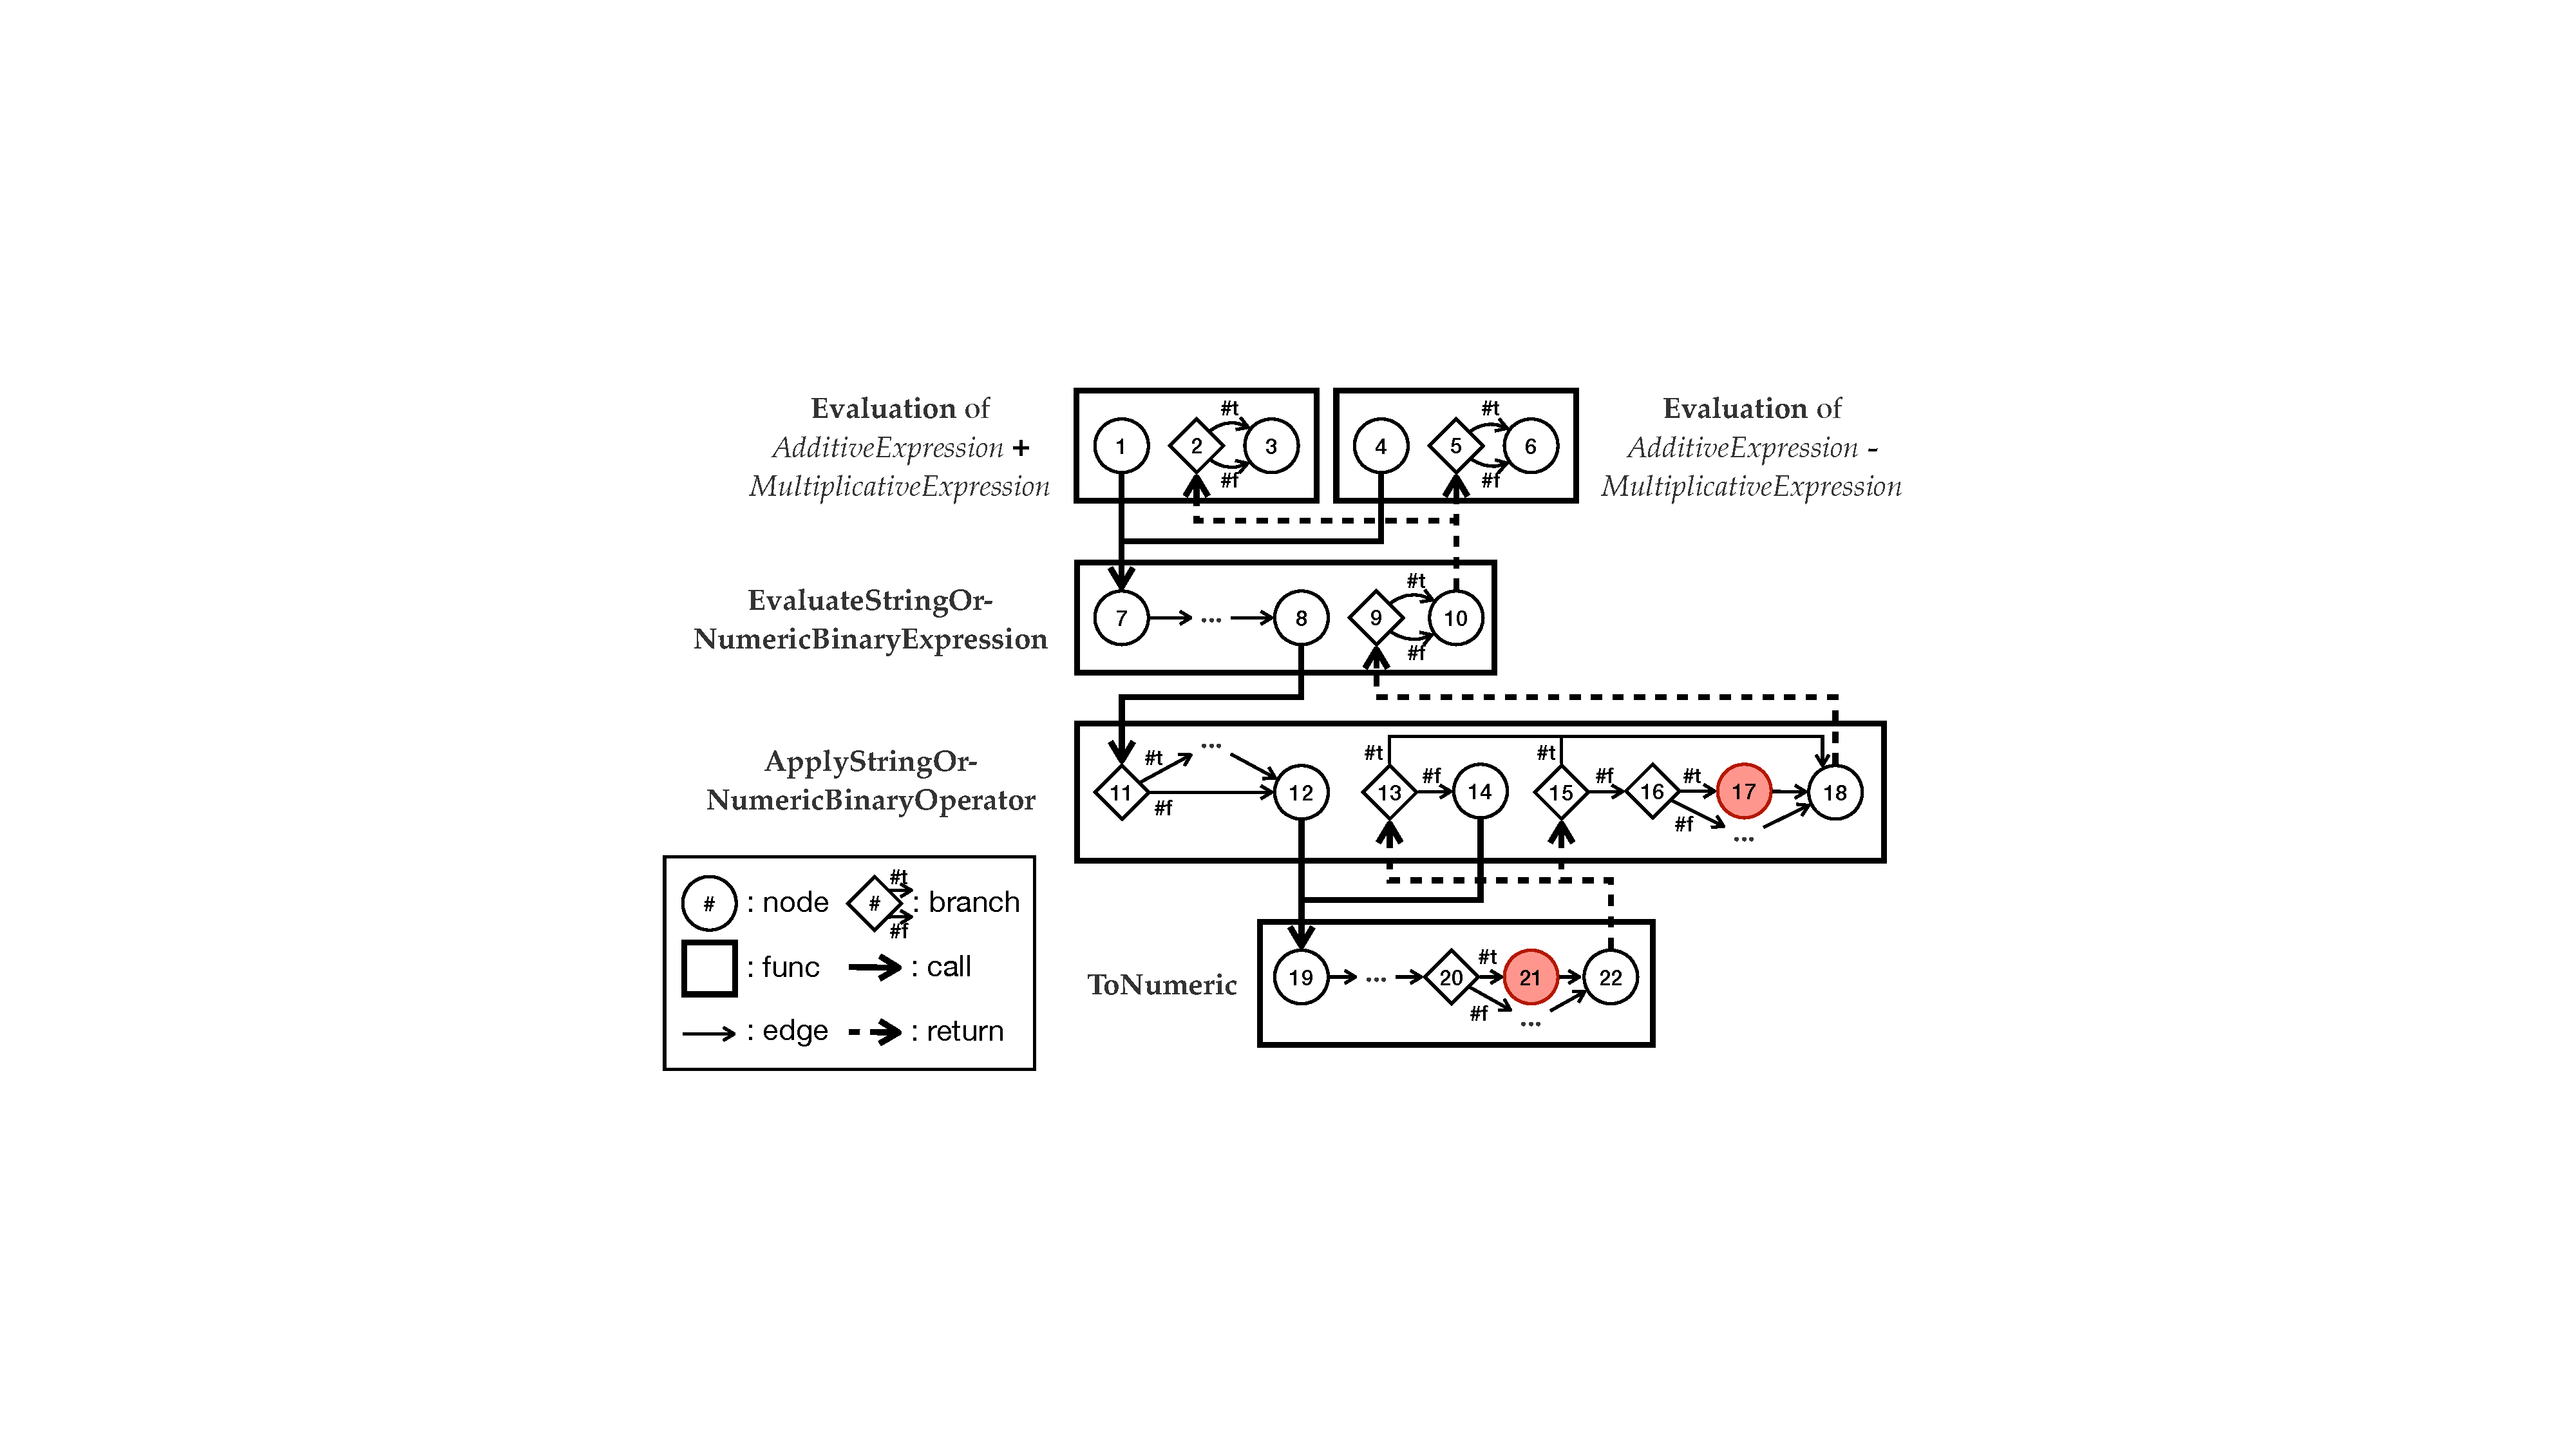
\includegraphics[width=\textwidth]{img/spec-cfg}
  \caption{
    The control-flow graph (CFG) of abstract algorithms in
    Figure~\ref{fig:add-sdo}, \ref{fig:normal-algos}, and
    \ref{fig:builtin-number}.
  }
  \label{fig:spec-cfg}
\end{figure}

Prior work~\cite{jest} presents a way to automatically synthesize JavaScript
conformance tests using coverage-guided fuzzing with the control-flow graph
(CFG) in the language specification.
%
It first utilizes another tool $\jiset$~\cite{jiset} to extract a mechanized
specification from a given version of ECMA-262.
%
A specification is mechanized when it is formally defined and executable.
%
Then, it constructs a CFG from the mechanized specification and performs
a coverage-guided fuzzing~\cite{afl} to synthesize diverse JavaScript programs.
%
To keep meaningful synthesized programs, it maintains a \textit{program pool}
based on coverage information of the programs in the extracted CFG.
%
It repeatedly tries to construct a new program by mutating programs in the pool
and adds the new mutated program to the pool when it covers more nodes or
branches.
%
Finally, it automatically injects assertions to the synthesized programs in the
pool to convert them to the conformance tests for JavaScript.
%
The assertions injected into each program represents the final state of its
execution on the mechanized specification.

%----------------------------------------%

For example, we could extract a CFG depicted in Figure~\ref{fig:spec-cfg} from
the abstract algorithms in Figures~\ref{fig:add-sdo}, \ref{fig:normal-algos},
and \ref{fig:builtin-number} via $\jiset$.
%
In this graph, circles denote nodes, diamonds denote branches, and boxes denote
algorithms.
%
Thin arrows indicate intra-algorithm control flows, but thick arrows indicate
inter-algorithm control flows: calls for solid arrows and returns for dotted
arrows.
%
The labels in nodes match the labels annotated in the algorithms.
%
Now, consider a simple JavaScript program: \jscode{let x = 1 + 2;}.
%
Then, it covers only the false branch of $20$ because the left- and right-hand
sides of \jscode{1 + 2} are both Number values rather than BitInt values.
%
In this case, the coverage-guided fuzzer repeatedly mutates it to cover the true
branch of $20$ and might get another program: \jscode{let x = 3n + 4n;}.
%
The new mutated program now covers the true branch of $20$ and the node of $21$.
%
Finally, the assertion \jscode{assert(x === 7n);} is automatically injected into
the mutated program based on the final state of its execution on the mechanized
specification.




\subsection{Motivation}

Prior work utilizes simple \textit{node/branch coverages} in the coverage-guided
fuzzer to synthesize JavaScript conformance tests.
%
However, such simple coverage metrics cannot fully discriminate different
semantics in different language features or even in the same features.
%
I explain such cases with simple examples in the CFG depicted in
Figure~\ref{fig:spec-cfg}.




\subsubsection{Different Semantics in Different Language Features}

Different language features might share the same abstract algorithms to define
their semantics.
%
For example, the semantics of addition (\scode{+}) and subtraction (\scode{-})
operators are defined with \textbf{EvaluateStringOrNumericBinaryExpression} and
other transitively related normal algorithms as helpers.
%
Now, assume that the current program pool is as follows:
\[
  \cdots \qquad \jscode{2n + 1;} \qquad \cdots
\]
%
Then, the node $17$ is covered by the program \jscode{2n + 1;} because it has
different types of numeric values, a BigInt \jscode{2n} and a Number {1}, as the
left- and right-hand sides of the addition operator (\scode{+}).
%
It means that another similar program \jscode{2n - 1;} might not be added to the
program pool because the test requirement for the node $17$ is already satisfied
by \jscode{2n + 1;}.
%
However, the conformance test inferred from \jscode{2n - 1;} is also a
meaningful test case that checks the edge case throwing a \textbf{TypeError}
exception in the semantics of the subtraction operator (\scode{-}).
%
It even lowers the chance of synthesizing more complex programs using the
subtraction operator (\scode{-}), such as \jscode{[] - ""}.
%
Therefore, we need a more fine-grained definition of test requirements that
discriminates \jscode{2n + 1;} and \jscode{2n - 1;} for a more advanced
JavaScript conformance test suite.



\subsubsection{Different Semantics in Same Language Features}

Moreover, different parts in the semantics of even the same language features
might be defined using the same algorithms.
%
For example, the semantics of the addition operator (\scode{+}) is defined with
\textbf{ApplyStringOrNumericBinaryOperator}, and it invokes \textbf{ToNumeric}
twice in the nodes 12 and 14.
%
Now, assume that the current program pool is as follows:
\[
  \cdots \qquad \jscode{2n + 1;} \qquad \cdots
\]
%
Then, the node $21$ is covered by the program: \jscode{2n + 1;} because the
left-hand side is a BigInt \jscode{2n}.
%
It means that another similar program \jscode{1 + 2n;} might not be added to the
program pool because the test requirement for the node $21$ is already satisfied
by \jscode{2n + 1;}.
%
However, the conformance test inferred from \jscode{1 + 2n;} is also a
meaningful test case to check the edge case when the right-hand side of the
addition operator (\scode{+}) is a BigInt value.

%----------------------------------------%

To resolve this problem, we propose a feature-sensitive coverage and its
variants to discriminate test requirements based on enclosing language features
in Section~\ref{sec:fscov}.
